\documentclass[a4paper,12pt]{article} 

%%% Работа с русским языком
\usepackage{cmap}					% поиск в PDF
\usepackage{mathtext} 				% русские буквы в фомулах
\usepackage[T2A]{fontenc}			% кодировка
\usepackage[utf8]{inputenc}			% кодировка исходного текста
\usepackage[english,russian]{babel}	% локализация и переносы

%%% Дополнительная работа с математикой
\usepackage{amsmath,amsfonts,amssymb,amsthm,mathtools, gensymb} % AMS
\usepackage{icomma} % "Умная" запятая: $0,2$ --- число, $0, 2$ --- перечисление

%%Таблица
\usepackage[table,xcdraw]{xcolor}
\usepackage{caption}
\usepackage{floatrow}
\floatsetup[table]{capposition=top}
\floatsetup[wrapfigure]{capposition=bottom}


%% Номера формул
\mathtoolsset{showonlyrefs=true} % Показывать номера только у тех формул, на которые есть \eqref{} в тексте.

%% Шрифты
\usepackage{euscript}	 % Шрифт Евклид
\usepackage{mathrsfs} % Красивый матшрифт

%% Свои команды
\DeclareMathOperator{\sgn}{\mathop{sgn}}

%% Перенос знаков в формулах (по Львовскому)
\newcommand*{\hm}[1]{#1\nobreak\discretionary{}
{\hbox{$\mathsurround=0pt #1$}}{}}

%% Стиль страницы
\usepackage{fancyhdr}

%% Для рисунков
\usepackage{graphicx}
\usepackage[export]{adjustbox}
\usepackage{float}
\usepackage{ragged2e}
\usepackage{wrapfig}

\pagestyle{fancy}
\begin{document}
\begin{titlepage}
\begin{center}
%\vspace*{1cm}
\large{\small ФЕДЕРАЛЬНОЕ ГОСУДАРСТВЕННОЕ АВТОНОМНОЕ ОБРАЗОВАТЕЛЬНОЕ\\ УЧРЕЖДЕНИЕ ВЫСШЕГО ОБРАЗОВАНИЯ \\ МОСКОВСКИЙ ФИЗИКО-ТЕХНИЧЕСКИЙ ИНСТИТУТ\\ (НАЦИОНАЛЬНЫЙ ИССЛЕДОВАТЕЛЬСКИЙ УНИВЕРСИТЕТ)\\ ФАКУЛЬТЕТ АЭРОКОСМИЧЕСКИХ ТЕХНОЛОГИЙ}
\vfill
\line(1,0){430}\\[1mm]
\huge{Лабораторная работа 2.2.2}\\
\huge\textbf{Измерение теплопроводности воздуха при разных давлениях}\\
\line(1,0){430}\\[1mm]
\vfill
\begin{flushright}
\normalsize{Рогозин Владимир}\\
\normalsize{\textbf{Группа Б03-105}}\\
\end{flushright}
\end{center}
\end{titlepage}
\fancyhead[L] {Работа 2.2.2}


\textbf{Цель работы}: исследовать теплопередачу от нагретой нити к цилиндрической оболочке в зависимости от концентрации (давления) заполняющего её воздуха. Измерить коэффициент теплопроводности при высоких давлениях; определить область перехода к режиму теплопередачи; определить коэффициент теплопередачи при низких давлениях.

\textbf{Оборудование}: цилиндрическая колба с натянутой по оси платиновой нитью; форвакуумный насос; вакуумметр; масляный манометр; вольтметр и амперметр
(цифровые мультиметры); источник постоянного тока.

\textbf{Теоретические сведения}: 

\begin{wrapfigure}[9]{}{0.6\textwidth}
    \begin{flushright}
    \vspace{-20pt}
        \includegraphics[width = \textwidth]{перенос.png}
    \end{flushright}
\end{wrapfigure}
\textit{Теплопроводность} — явление переноса, процесс передачи энергии от нагретых частей системы к холодным за счёт хаотического движения частиц среды.
В газах теплопроводность осуществляется за счёт непосредственной передачи кинетической энергии от быстрых молекул к медленным при их столкновениях.
Перенос тепла описывается законом Фурье, утверждающим, что плотность потока энергии $\Vec{q}$ (количество теплоты, переносимое через единичную площадку в единицу времени) пропорциональна градиенту температуры $\nabla T$. 
\[\Vec{q} = -\varkappa\nabla T\]
где $\varkappa$ -- \textit{коэффициент теплопроводности.}
В данной работе система имеет цилиндрическую симметрию: можно считать, что все параметры газа зависят только от расстояния до оси системы $r$. Тогда имеем:
\[q = -\varkappa\frac{dT}{dr}\]
Система, в которой имеются перепады температур, не находится в состоянии равновесия. Говоря о зависимости температуры от координат $T(r)$ мы
подразумеваем, что систему можно разбить элементарные подсистемы, в каждой из которых имеет место \textit{локальное тепловое равновесие}. В газах закон Фурье применим, если характерный размер $r$ задачи превосходит \textit{длину свободного пробега} молекул: $\lambda \ll r$, а температура меняется
незначительно на масштабах длины пробега: $\lambda|\nabla T|\ll T$.

Для количественного описания способности некоторой системы к теплопередаче в целом (независимо от её механизма) используют коэффициент, называемый \textit{тепловым сопротивлением}, равный отношению перепада температур $\Delta T$ в системе к полному потоку энергии $Q$ через неё:
\[K = \frac{\Delta T}{Q}\]
(по аналогии с электрической цепью, где $\Delta T$ -- аналог напряжения, а $Q$ -- тока).

Закон Фурье применим только в случае плотных газов, при таком условии теоретическая оценка даёт выражение для коэффициента теплопроводности:
\[\varkappa \approx \frac{1}{3}\lambda \overline{v}\cdot n C_{V}\]
где n -- концентрация молекул газа, $\overline{v} = \sqrt{\frac{8RT}{\pi\mu}}$ -- средняя скорость теплового движения молекул, $С_{V} = \frac{i}{2} k_{Б}$ -- теплоёмкость при постоянном объёме для одной молекулы (i -- эффективное число степеней свободы молекулы).

Длина свободного пробега обратно пропорциональна $ n : \lambda = 1 / n\sigma,\text{ } \sigma$ -- эффективное сечение столкновений молекул друг с другом есть величина, характеризующая вероятность отклонения налетающих частиц при взаимодействии с некоторым рассеивающим центром. В общем случае она определяется как отношение полного потока рассеянных частиц к плотности потока падающих, и имеет размерность площади. В простейшем случае одинаковых твёрдых шариков $\sigma = \pi d^2 $, где $d$ -- диаметр шариков, поэтому коэффициент теплопроводности газа \textit{не зависит} от его концентрации (а значит, и от давления) и определяется только его температурой.

В случае разреженного газа, когда  длина свободного пробега молекул относительно столкновений друг с другом $\lambda$ превосходит характерные размеры системы: $\lambda \gtrsim r$. Тогда молекулы сталкиваются в
основном не между собой, а со стенками. При этом теряет смысл понятие
температуры как функции координат и, следовательно, градиента температуры, так что закон Фурье становится неприменим. Если в системе есть
поверхности, находящиеся при разных температурах, процесс обмена энергией между ними за счёт молекул газа, заполняющего сосуд, принято называть \textit{теплопередачей} (возможен также теплообмен за счёт \textit{излучения}). Молекулы при неупругих ударах о нагретую поверхность приобретают среднюю кинетическую энергию, соответствующую температуре этой поверхности; отразившись от неё и не сталкиваясь с другими молекулами, они долетают до холодной поверхности и передают ей избыточную энергию. Отметим, что такое состояние газа является \textit{неравновесным}, поэтому температура самого газа, строго говоря, не определена.

Рассмотрим упрощённую модель теплопередачи в цилиндрическом сосуде радиуса $R$ и длины $L$ ($L \gg R$) 
на оси которого натянута тонкая нить радиуса $r_н$ ($r_н \ll R$). Пусть температуры колбы и нити равны $T_к$ и $T_н$ соответственно ($T_н > T_н$) . Предположим сначала, что длина свободного пробега превосходит радиус колбы $\lambda \gtrsim R$.

Все молекулы в пространстве колбы можно разделить на две группы: в зависимости от того, с какой поверхностью — с колбой или с нитью — они испытали последнее
неупругое столкновение, их средняя энергия равна $c_V T_к$, либо $c_V T_н$ соответственно. В \textit{стационарном} состоянии потоки частиц, падающих на нить и улетающих от неё, равны. Полный поток падающих на нить частиц составляет
\[J = \frac{1}{4} n \overline{v}\cdot S_{н}\]
где n -- концентрация частиц, $\overline{v}$ -- средняя скорость их теплового движения, $S = 2\pi r_н L$ -- площадь поверхности нити. В данной работе относительный перепад температур мал, поэтому при расчёте потока частиц можно не различать средние скорости «горячих» (летящих от нити) и «холодных» (летящих к нити) частиц.

Учтём, что не все столкновения молекул с нитью или стенками колбы являются неупругими (при упругом отражении молекула не передаёт энергию стенке). Для этого введём поправочный множитель $s$, называемый коэффициентом аккомодации. Он пропорционален вероятности неупругого удара, которая определяется структурой и материалом поверхности и, вообще говоря, может зависеть от $T$, однако при $\Delta T \ll T$ его можно считать постоянным.

Таким образом суммарный поток энергии от нити к стенкам колбы в единицу времени будет равен
\[Q \approx \frac{1}{4} s S_н n \overline{v}\cdot c_{V} (T_н - T_к) \]
Отсюда тепловое сопротивление равняется 
\begin{equation}\label{eq:sostoyanie_teploperedachi}
    \frac{1}{K_т} = \frac{1}{4} s S_н n \overline{v}\cdot c_{V}
\end{equation}

В отличие от случая плотного газа, интенсивность теплопередачи обратно пропорциональна концентрации газа в колбе. Также, в таком режиме роль длины свободного пробега играет радиус нити $r_н$
\[\frac{1}{K_тL} \sim r_н \overline{v}\cdot n c_V\]

Рассмотрим самый общий случай. При больших $n$ длина свободного пробега меньше радиуса нити, поэтому реализуется режим \textit{теплопроводности}. По мере уменьшения давления уменьшается и концентрация газа ($P = n \cdot k_Б T$), когда длина свободного пробега примерно становится равной радиусу нити $r_н$ вблизи нити появляется область теплопередачи размером $\sim \lambda$, в которой закон Фурье неприменим. 

Пусть на нити выделяется известная мощность $Q$. Тогда в области \textit{теплопроводности} имеем 
\[Q = -2\pi r L\cdot\varkappa\frac{dT}{dr}, \text{ }(r_н + \lambda\leq r \leq R )\]
Так как в этой работе перепад температур мал ($\Delta T \ll T_к$), то можно положить, что в условиях эксперимента теполпроводность остаётся постоянной $\varkappa \approx \varkappa(T_к)$, отсюда интегрированием получем
\begin{equation}\label{eq:perepad_daleko_ot_niti}
    T(r) - T_к = \frac{Q}{2\pi L\varkappa}\ln{\frac{R}{r}}
\end{equation}
Вблизи нити имеем
\begin{equation}\label{eq:perepad_vblizi_niti}
    T_н - T(r_н + \lambda) = K_т\cdot Q
\end{equation}
где $K_т$ -- тепловое сопротивление в области теплопередачи, определяемое формулой \eqref{eq:sostoyanie_teploperedachi}, $T(r_н + \lambda)$ -- температура на границе этой области. С помощью этих двух уравнений, подставив $r = r_н + \lambda$ в уравнение \eqref{eq:perepad_daleko_ot_niti} найдём разность температур нити и колбы 
\[\Delta T = \frac{Q}{2\pi L\varkappa}\ln{\frac{R}{r_н + \lambda}} + K_т\cdot Q\]

Проанализируем логарифм в последнем выражении, при больших давлениях ($\lambda \ll r_н$) длиной свободного пробега в знаменателе логарифмма можно пренебречь, с другой стороны, при малых давлениях ($\lambda \gg r_н$) логарифмическая зависимость будет незаметна на фоне слагаемого $K_т$, которое возрастает согласно \eqref{eq:sostoyanie_teploperedachi} как $\frac{1}{n}$, значит можно положить $\ln{\frac{R}{r_н + \lambda}} \approx \ln{\frac{R}{r_н}}$. Учитывая, что измеряемой величиной будет давление $P$, формулу для перепада температур можно переписать в виде 
\[\Delta T = Q (K + \frac{A}{P})\]
где $K$ и $A$ -- постоянные, которые могут быть определены экспериментально. Величина $K$ есть тепловое сопротивление системы при высоких давлениях, по его значению можно вычислить коэффициент теплопроводности газа $\varkappa$. По значению $A$ можно определить коэффициент аккомодации $s$ и таким образом найти тепловое сопротивление системы при любом давлении
\[K^{'} = \frac{\Delta T}{Q} = K + \frac{A}{P}\]

\textbf{Экспериментальная установка}: Схема установки приведена на картинке ниже. Внутренняя полость тонкостенной цилиндрической стеклянной колбы, на оси которой натянута платиновая нить, подсоединена к вакуумной установке. Колба заполнена воздухом и расположена вертикально.
\begin{figure}[H]
    \label{fig:ustanovka}
    \centering
    \includegraphics[width = 0.7\textwidth]{установка.png}
    \caption{Вакуумная часть экспериментальной устнаовки}
\end{figure}

\begin{wrapfigure}[6]{}{0.4\textwidth}
    \begin{flushright}
        \vspace{-45pt}
        \includegraphics[width = \textwidth]{мерить сопротивление.png}
    \end{flushright}
\end{wrapfigure}

Диаметр нити $2r_н = 0,05$ мм, диаметр колбы $2R = 10$ мм($\ln{\frac{R}{r_н}}\approx 5,3$), длина нити $L = 220$ мм.

Металлическая нить служит как источником тепла, так и датчиком температуры (термометром сопротивления). В рабочем диапазоне температур (20–40 ℃) сопротивление платины зависит от температуры практически линейно:
\[R(t) = R_0(1 + \alpha_0t)\]
где $t$ -- температура в \degree C, $R_0$ -- сопротивление при 0\degree C, и 
\[\alpha_0 = \frac{1}{R_0}\frac{dR}{dt} = 3,92\cdot 10^{-3} \text{ }\degree C^{-1}\] -- \textit{температурный коэффициент сопротивления} платины в указанном температурном диапазоне.

\textbf{Обработка данных}: Все измерения производились при атмосферном давлении $P_{атм} = 100,5 \text{ }КПа$, и комнатной температуре $T_{комн} = 296,9 \text{ }К$. Ниже представлены результаты измерений перепада напряжения и сила тока на участке нити при различных давлениях:
\begin{table}[H]\label{tab:p_s_atm}
    \centering
    \begin{tabular}{|cc|cc|cc|cc|}
        \hline
        \multicolumn{2}{|c|}{{\color[HTML]{000000} $P = P_{атм}$}} &
          \multicolumn{2}{c|}{{\color[HTML]{000000} $P = 21,5 \text{ }КПа$}} &
          \multicolumn{2}{c|}{{\color[HTML]{000000} $P = 50,5 \text{ }КПа$}} &
          \multicolumn{2}{c|}{{\color[HTML]{000000} $P = 80,5 \text{ }КПа$}} \\ \hline
        \multicolumn{1}{|c|}{{\color[HTML]{000000} $I, мА$}} &
          {\color[HTML]{000000} $U, мВ$} &
          \multicolumn{1}{c|}{{\color[HTML]{000000} $I, мА$}} &
          {\color[HTML]{000000} $U, мВ$} &
          \multicolumn{1}{c|}{{\color[HTML]{000000} $I, мА$}} &
          {\color[HTML]{000000} $U, мВ$} &
          \multicolumn{1}{c|}{{\color[HTML]{000000} $I, мА$}} &
          {\color[HTML]{000000} $U, мВ$} \\ \hline
        \multicolumn{1}{|c|}{{\color[HTML]{000000} 10,00}} &
          {\color[HTML]{000000} 116,795} &
          \multicolumn{1}{c|}{{\color[HTML]{000000} 10,00}} &
          {\color[HTML]{000000} 118,236} &
          \multicolumn{1}{c|}{{\color[HTML]{000000} 10,00}} &
          {\color[HTML]{000000} 118,272} &
          \multicolumn{1}{c|}{{\color[HTML]{000000} 10,04}} &
          {\color[HTML]{000000} 118,600} \\ \hline
        \multicolumn{1}{|c|}{{\color[HTML]{000000} 18,00}} &
          {\color[HTML]{000000} 210,347} &
          \multicolumn{1}{c|}{{\color[HTML]{000000} 18,00}} &
          {\color[HTML]{000000} 213,015} &
          \multicolumn{1}{c|}{{\color[HTML]{000000} 18,11}} &
          {\color[HTML]{000000} 214,420} &
          \multicolumn{1}{c|}{{\color[HTML]{000000} 18,13}} &
          {\color[HTML]{000000} 214,363} \\ \hline
        \multicolumn{1}{|c|}{{\color[HTML]{000000} 26,01}} &
          {\color[HTML]{000000} 304,630} &
          \multicolumn{1}{c|}{{\color[HTML]{000000} 26,12}} &
          {\color[HTML]{000000} 309,505} &
          \multicolumn{1}{c|}{{\color[HTML]{000000} 26,12}} &
          {\color[HTML]{000000} 309,740} &
          \multicolumn{1}{c|}{{\color[HTML]{000000} 26,13}} &
          {\color[HTML]{000000} 311,092} \\ \hline
        \multicolumn{1}{|c|}{{\color[HTML]{000000} 32,04}} &
          {\color[HTML]{000000} 376,060} &
          \multicolumn{1}{c|}{{\color[HTML]{000000} 32,20}} &
          {\color[HTML]{000000} 382,190} &
          \multicolumn{1}{c|}{{\color[HTML]{000000} 32,22}} &
          {\color[HTML]{000000} 382,820} &
          \multicolumn{1}{c|}{{\color[HTML]{000000} 32,04}} &
          {\color[HTML]{000000} 382,209} \\ \hline
        \multicolumn{1}{|c|}{{\color[HTML]{000000} 40,05}} &
          {\color[HTML]{000000} 471,681} &
          \multicolumn{1}{c|}{{\color[HTML]{000000} 40,02}} &
          {\color[HTML]{000000} 476,490} &
          \multicolumn{1}{c|}{{\color[HTML]{000000} 40,33}} &
          {\color[HTML]{000000} 480,600} &
          \multicolumn{1}{c|}{{\color[HTML]{000000} 40,08}} &
          {\color[HTML]{000000} 479,740} \\ \hline
        \multicolumn{1}{|c|}{{\color[HTML]{000000} 48,10}} &
          {\color[HTML]{000000} 568,630} &
          \multicolumn{1}{c|}{{\color[HTML]{000000} 48,06}} &
          {\color[HTML]{000000} 574,526} &
          \multicolumn{1}{c|}{{\color[HTML]{000000} 48,02}} &
          {\color[HTML]{000000} 574,590} &
          \multicolumn{1}{c|}{{\color[HTML]{000000} 48,02}} &
          {\color[HTML]{000000} 576,930} \\ \hline
        \multicolumn{1}{|c|}{{\color[HTML]{000000} 56,09}} &
          {\color[HTML]{000000} 665,950} &
          \multicolumn{1}{c|}{{\color[HTML]{000000} 56,80}} &
          {\color[HTML]{000000} 684,480} &
          \multicolumn{1}{c|}{{\color[HTML]{000000} 56,13}} &
          {\color[HTML]{000000} 675,090} &
          \multicolumn{1}{c|}{{\color[HTML]{000000} 56,14}} &
          {\color[HTML]{000000} 678,260} \\ \hline
        \multicolumn{1}{|c|}{{\color[HTML]{000000} 62,22}} &
          {\color[HTML]{000000} 742,660} &
          \multicolumn{1}{c|}{{\color[HTML]{000000} }} &
          {\color[HTML]{000000} } &
          \multicolumn{1}{c|}{{\color[HTML]{000000} }} &
          {\color[HTML]{000000} } &
          \multicolumn{1}{c|}{{\color[HTML]{000000} }} &
          {\color[HTML]{000000} } \\ \hline
    \end{tabular}
    \caption*{Данные для давлений, близких к атмосферному}
\end{table}
\begin{table}[H]\label{tab:p_malenkiye}
    \centering
    \begin{tabular}{|cc|cc|cc|cc|}
        \hline
        \multicolumn{2}{|c|}{{\color[HTML]{000000} $P = 292,05 \text{ }Па$}} &
          \multicolumn{2}{c|}{{\color[HTML]{000000} $P = 557,55 \text{ }Па$}} &
          \multicolumn{2}{c|}{{\color[HTML]{000000} $P = 823,05 \text{ }Па$}} &
          \multicolumn{2}{c|}{{\color[HTML]{000000} $P = 1504,50 \text{ }Па$}} \\ \hline
        \multicolumn{1}{|c|}{{\color[HTML]{000000} $I, мА$}} &
          {\color[HTML]{000000} $U, мВ$} &
          \multicolumn{1}{c|}{{\color[HTML]{000000} $I, мА$}} &
          {\color[HTML]{000000} $U, мВ$} &
          \multicolumn{1}{c|}{{\color[HTML]{000000} $I, мА$}} &
          {\color[HTML]{000000} $U, мВ$} &
          \multicolumn{1}{c|}{{\color[HTML]{000000} $I, мА$}} &
          {\color[HTML]{000000} $U, мВ$} \\ \hline
        \multicolumn{1}{|c|}{{\color[HTML]{000000} 10,00}} &
          {\color[HTML]{000000} 117,251} &
          \multicolumn{1}{c|}{{\color[HTML]{000000} 10,00}} &
          {\color[HTML]{000000} 117,293} &
          \multicolumn{1}{c|}{{\color[HTML]{000000} 10,00}} &
          {\color[HTML]{000000} 117,487} &
          \multicolumn{1}{c|}{{\color[HTML]{000000} 10,04}} &
          {\color[HTML]{000000} 118,747} \\ \hline
        \multicolumn{1}{|c|}{{\color[HTML]{000000} 18,14}} &
          {\color[HTML]{000000} 212,872} &
          \multicolumn{1}{c|}{{\color[HTML]{000000} 18,14}} &
          {\color[HTML]{000000} 213,026} &
          \multicolumn{1}{c|}{{\color[HTML]{000000} 18,15}} &
          {\color[HTML]{000000} 213,360} &
          \multicolumn{1}{c|}{{\color[HTML]{000000} 18,12}} &
          {\color[HTML]{000000} 214,556} \\ \hline
        \multicolumn{1}{|c|}{{\color[HTML]{000000} 26,11}} &
          {\color[HTML]{000000} 307,861} &
          \multicolumn{1}{c|}{{\color[HTML]{000000} 26,18}} &
          {\color[HTML]{000000} 308,022} &
          \multicolumn{1}{c|}{{\color[HTML]{000000} 26,15}} &
          {\color[HTML]{000000} 308,125} &
          \multicolumn{1}{c|}{{\color[HTML]{000000} 26,14}} &
          {\color[HTML]{000000} 310,159} \\ \hline
        \multicolumn{1}{|c|}{{\color[HTML]{000000} 32,25}} &
          {\color[HTML]{000000} 380,331} &
          \multicolumn{1}{c|}{{\color[HTML]{000000} 32,13}} &
          {\color[HTML]{000000} 379,034} &
          \multicolumn{1}{c|}{{\color[HTML]{000000} 32,02}} &
          {\color[HTML]{000000} 380,577} &
          \multicolumn{1}{c|}{{\color[HTML]{000000} 32,24}} &
          {\color[HTML]{000000} 383,520} \\ \hline
        \multicolumn{1}{|c|}{{\color[HTML]{000000} 40,07}} &
          {\color[HTML]{000000} 474,306} &
          \multicolumn{1}{c|}{{\color[HTML]{000000} 40,05}} &
          {\color[HTML]{000000} 474,151} &
          \multicolumn{1}{c|}{{\color[HTML]{000000} 40,06}} &
          {\color[HTML]{000000} 477,448} &
          \multicolumn{1}{c|}{{\color[HTML]{000000} 40,15}} &
          {\color[HTML]{000000} 479,692} \\ \hline
        \multicolumn{1}{|c|}{{\color[HTML]{000000} 48,00}} &
          {\color[HTML]{000000} 570,900} &
          \multicolumn{1}{c|}{{\color[HTML]{000000} 48,09}} &
          {\color[HTML]{000000} 571,964} &
          \multicolumn{1}{c|}{{\color[HTML]{000000} 48,00}} &
          {\color[HTML]{000000} 574,415} &
          \multicolumn{1}{c|}{{\color[HTML]{000000} 48,00}} &
          {\color[HTML]{000000} 575,600} \\ \hline
        \multicolumn{1}{|c|}{{\color[HTML]{000000} 56,12}} &
          {\color[HTML]{000000} 671,451} &
          \multicolumn{1}{c|}{{\color[HTML]{000000} 56,07}} &
          {\color[HTML]{000000} 670,715} &
          \multicolumn{1}{c|}{{\color[HTML]{000000} 56,11}} &
          {\color[HTML]{000000} 674,950} &
          \multicolumn{1}{c|}{{\color[HTML]{000000} 56,00}} &
          {\color[HTML]{000000} 674,370} \\ \hline
    \end{tabular}
    \caption*{Данные для малых давлений}
\end{table}
\newpage
Далее пострим график зависимости $R(Q)$ при атмсоферном давлении, оттуда найдём значение сопротивления при комнатной температуре. При комнатной температуре $Q = 0$, следовательно $R_0 = R_{к} / (1 + \alpha_0 t_{к})$.

\begin{figure}[H]\label{fig:R(Q)_atm}
    \centering
    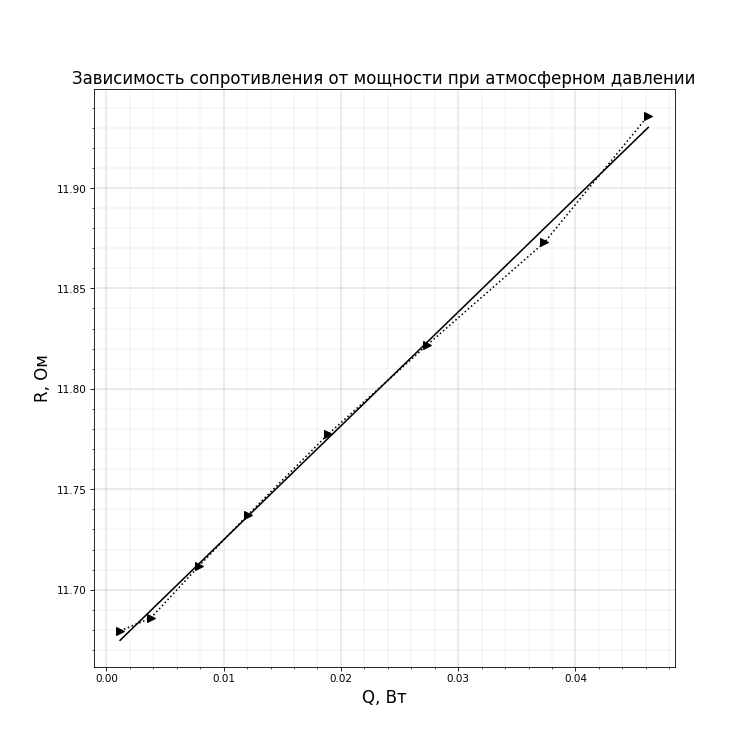
\includegraphics[width = \textwidth]{R(Q)_atm.png}
\end{figure}
\[R = a\cdot Q + b, \text{ }R(0) = b = R_к\]
Из графика находим 
\[b = (11,67\pm 0,0014)Ом = R_к, \text{ }\varepsilon_{R_к} \approx 0,01 \% \]
\[R_0 = (10,67 \pm 0.0011)Ом,\text{ }\varepsilon_{R_0} \approx 0,01 \%\]

Далее, построим графики зависимости $T(Q)$ для каждого из давлений, по угловым коэффициентам рассчитаем тепловое сопротивление $K = \frac{dT}{dQ}$.
\begin{figure}[H]\label{fig:T(Q)_atm}
    \centering
    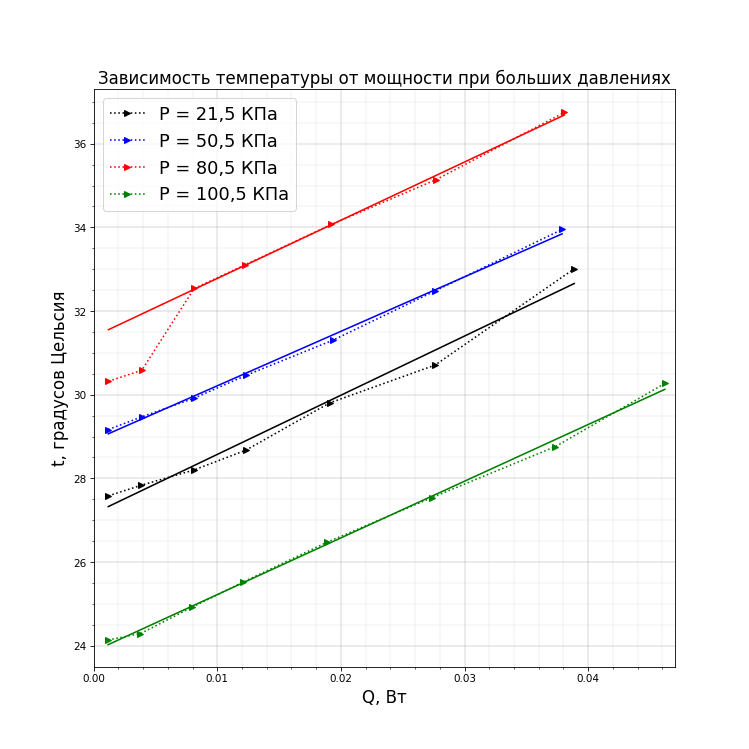
\includegraphics[width = \textwidth]{T(Q)_atm.png}
\end{figure}
Некоторые прямые на графике для удобства были подняты на константу, которая никак не влияет на угол наклона, при этом $T(0) = T_к$ были вычислены для неизменённых значений:

1) $P = 21,5$ КПа, $K = (141,48 \pm 7,17)\text{ }\degree C\cdot {Вт}^{-1}, \text{ }\varepsilon_K = 5,07\%, \text{ }\\ T(0) = T_к = (27,16 \pm 0,09)\text{ }\degree C, \text{ }\varepsilon_K = 0,33\%$

2) $P = 50,5$ КПа, $K = (130,22 \pm 2,51)\text{ }\degree C\cdot {Вт}^{-1}, \text{ }\varepsilon_K = 1,93\%, \text{ }\\ T(0) = T_к = (27,41 \pm 0,03)\text{ }\degree C, \text{ }\varepsilon_K = 0,11\%$

3) $P = 80,5$ КПа, $K = (139,15 \pm 2,25)\text{ }\degree C\cdot {Вт}^{-1}, \text{ }\varepsilon_K = 1,62\%, \text{ }\\ T(0) = T_к = (28,39 \pm 0,02)\text{ }\degree C, \text{ }\varepsilon_K = 0,07\%$

4) $P = 100,5$ КПа, $K = (135,53 \pm 2,22)\text{ }\degree C\cdot {Вт}^{-1}, \text{ }\varepsilon_K = 1,64\%, \text{ }\\ T(0) = T_к = (23,87 \pm 0,03)\text{ }\degree C, \text{ }\varepsilon_K = 0,13\%$

\begin{figure}[H]\label{fig:T(Q)_malo}
    \centering
    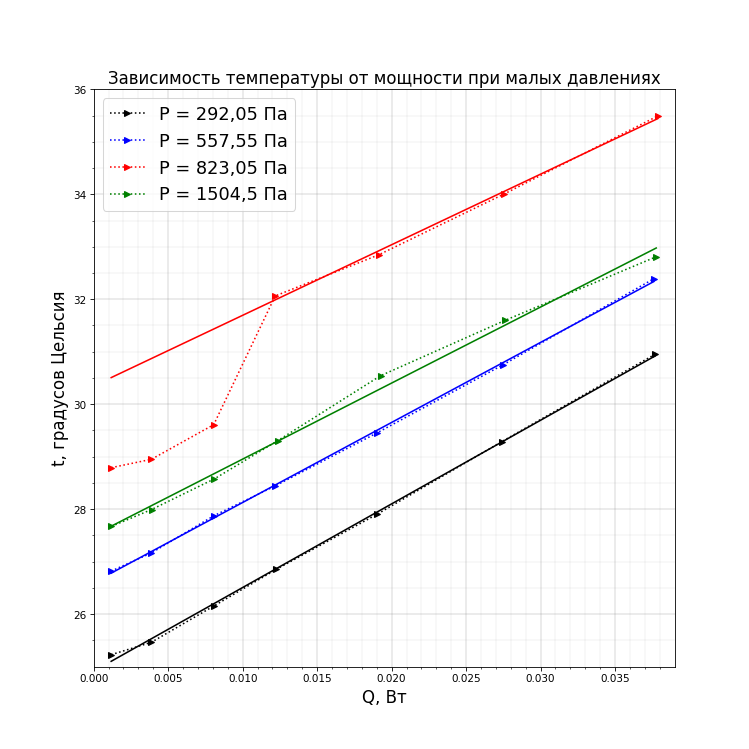
\includegraphics[width = \textwidth]{T(Q)_malo.png}
\end{figure}

На втором графике также некоторые прямые смещены на константу, значения $T(0) = T_к$ также вычислены для неизменённых значений:

1) $P = 292,05$ Па, $K = (159,37 \pm 1,86)\text{ }\degree C\cdot {Вт}^{-1}, \text{ }\varepsilon_K = 1,17\%, \text{ }\\ T(0) = T_к = (24,91 \pm 0,02)\text{ }\degree C, \text{ }\varepsilon_K = 0,08\%$

2) $P = 557,55$ Па, $K = (152,56 \pm 1,24)\text{ }\degree C\cdot {Вт}^{-1}, \text{ }\varepsilon_K = 0,81\%, \text{ }\\ T(0) = T_к = (25,11 \pm 0,02)\text{ }\degree C, \text{ }\varepsilon_K = 0,08\%$

3) $P = 823,05$ Па, $K = (134,51 \pm 3,33)\text{ }\degree C\cdot {Вт}^{-1}, \text{ }\varepsilon_K = 2,48\%, \text{ }\\ T(0) = T_к = (27,35 \pm 0,03)\text{ }\degree C, \text{ }\varepsilon_K = 0,11\%$

4) $P = 1504,5$ Па, $K = (144,90 \pm 3,91)\text{ }\degree C\cdot {Вт}^{-1}, \text{ }\varepsilon_K = 2,70\%, \text{ }\\ T(0) = T_к = (27,50 \pm 0,05)\text{ }\degree C, \text{ }\varepsilon_K = 0,18\%$
\newpage
Далее, построим график зависимости $K(lnP)$. 

\begin{figure}[H]\label{fig:K(lnP)}
    \centering
    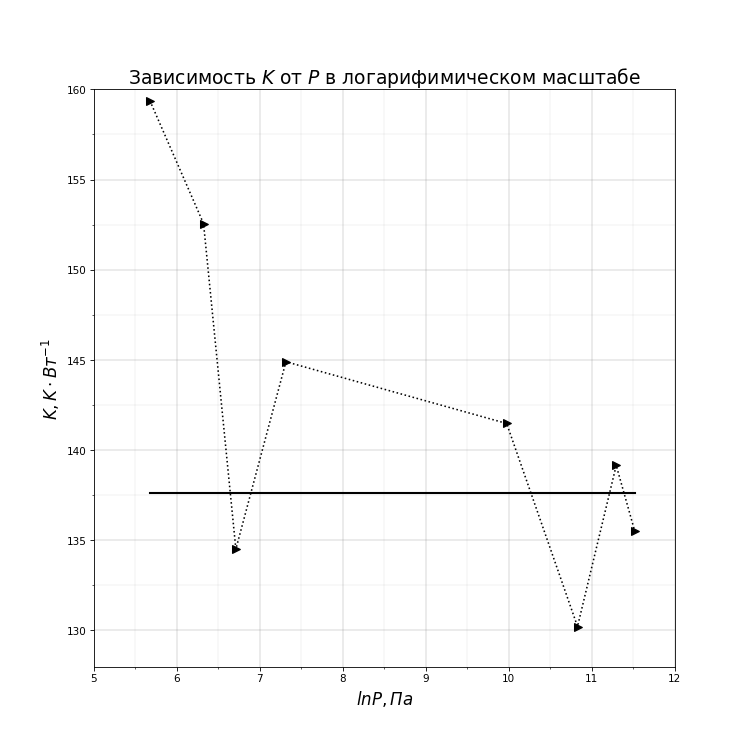
\includegraphics[width = \textwidth]{K_lnP.png}
\end{figure}
На графике видна область резкого возрастания теплового сопротивления, и примерно видна область $K = const$. С помощью горизонтального участка найдём коэффициент теплопроводности $\varkappa$:
\[K = const = (137,63 \pm 4,63)\text{ }\degree C\cdot {Вт}^{-1},\text{ } \varepsilon = 3,36\%\]
\[K = \frac{\Delta T}{Q} = \frac{1}{2\pi \varkappa L}\cdot \ln{\frac{R}{r_н}}\]
\[\varkappa = \frac{1}{2\pi K L}\ln{\frac{R}{r_н}} = (28 \pm 1)\cdot 10^{-3}\text{ }Вт/(м\cdotград), \text{ }\varepsilon_\varkappa = 3,36\%\]
Табличное значение теплопроводности воздуха при нормальных условиях равно
\[\varkappa_{табл} = 25,9 \cdot10^{-3}\text{ }Вт/(м\cdotград)\]

Затем, построим график зависимости $K(1/P)$, оттуда сможем найти коэффициент аккомодации $s$.
\begin{figure}[H]\label{fig:K(1/P)}
    \centering
    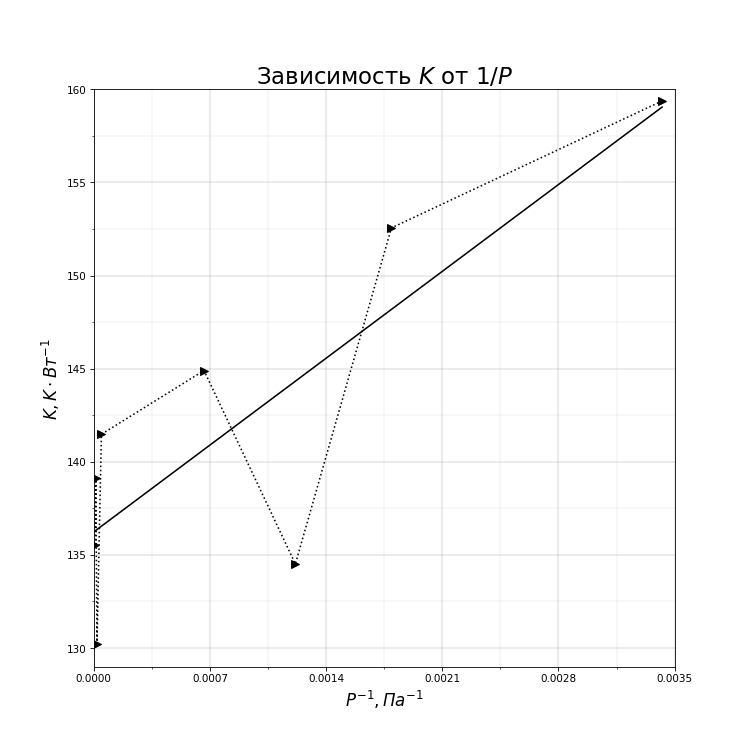
\includegraphics[width = \textwidth]{K_P-1.png}
\end{figure}
\[k = (6663,87 \pm 1566,61) \text{ }K\cdot Па \text{ }Вт^{-1}, \text{ }\varepsilon \approx 23,51\%\]
\[s = \frac{4}{5}\cdot \frac{T}{k \overline{v}\pi r_н L} = 4,41 \pm 1,04, \text{ }\varepsilon = 23,51\%\]
Табличное значение для коэффициента аккомодации
\[s_{табл} = 0,8 - 0,9\]


\textbf{Вывод}: В данной работе было исследовано явление теплопроводности воздуха, была изучена зависимость теплового сопротивления от давления, а также был вычислен коэффициент теплопроводности воздуха при нормальных условиях (результат почти сошёлся с табличным значением), и был вычислен коэффициент аккомодации воздуха (результат совсем не сошёлся с табличным значением).

\end{document}

